\documentclass[10pt]{beamer}
\usepackage[utf8]{inputenc}
\usepackage{xeCJK}
\usepackage{graphicx}
\usepackage{xcolor}
\usepackage {mathtools}
\usepackage{utopia} %font utopia imported
\usetheme{CambridgeUS}
\usecolortheme{dolphin}

% set colors
\definecolor{myNewColorA}{RGB}{25,25,112}
\definecolor{myNewColorB}{RGB}{25,25,112}
\definecolor{myNewColorC}{RGB}{25,25,112}
\setbeamercolor*{palette primary}{bg=myNewColorC}
\setbeamercolor*{palette secondary}{bg=myNewColorB, fg = white}
\setbeamercolor*{palette tertiary}{bg=myNewColorA, fg = white}
\setbeamercolor*{titlelike}{fg=myNewColorA}
\setbeamercolor*{title}{bg=myNewColorA, fg = white}
\setbeamercolor*{item}{fg=myNewColorA}
\setbeamercolor*{caption name}{fg=myNewColorA}
\usefonttheme{professionalfonts}
\usepackage{natbib}
\usepackage{hyperref}
\usepackage[absolute,overlay]{textpos}
\usepackage{graphicx}

\usepackage[italian]{babel}
%------------------------------------------------------------
\titlegraphic{
\includegraphics[height=2cm]{cherubino_pant541.eps}} 





\setbeamerfont{title}{size=\Large}
\setbeamerfont{subtitle}{size=\small}
\setbeamerfont{author}{size=\normalsize}
\setbeamerfont{date}{size=\footnotesize}
\setbeamerfont{institute}{size=\large}

\title[Università di Pisa]{Impiego di transmoni superconduttori\\
per la rivelazione
di assioni e materia oscura}

\author[Lorenzo Zaffina]{Candidato: Lorenzo Zaffina\\ Relatore: Prof. Gianluca Lamanna}


\institute[]{Università di Pisa\\
Dipartimento di Fisica "Enrico Fermi"}

\date[\textcolor{white}{15 settembre 2022} ]{Anno Accademico 2021-2022}


%------------------------------------------------------------
%This block of commands puts the table of contents at the 
%beginning of each section and highlights the current section:
%\AtBeginSection[]
%{
%  \begin{frame}
%    \frametitle{Contents}
%    \tableofcontents[currentsection]
%  \end{frame}
%}
\AtBeginSection[]{
  \begin{frame}
  \vfill
  \centering
  \begin{beamercolorbox}[sep=8pt,center,shadow=true,rounded=true]{title}
    \usebeamerfont{title}\insertsectionhead\par%
  \end{beamercolorbox}
  \vfill
  \end{frame}
}
%------------------------------------------------------------

\begin{document}

%The next statement creates the title page.
\frame{\titlepage}
\begin{frame}
\frametitle{Gli assioni: candidati per la materia oscura}



\begin{textblock*}{5cm}(8.1cm,2cm) % {block width} (coords)
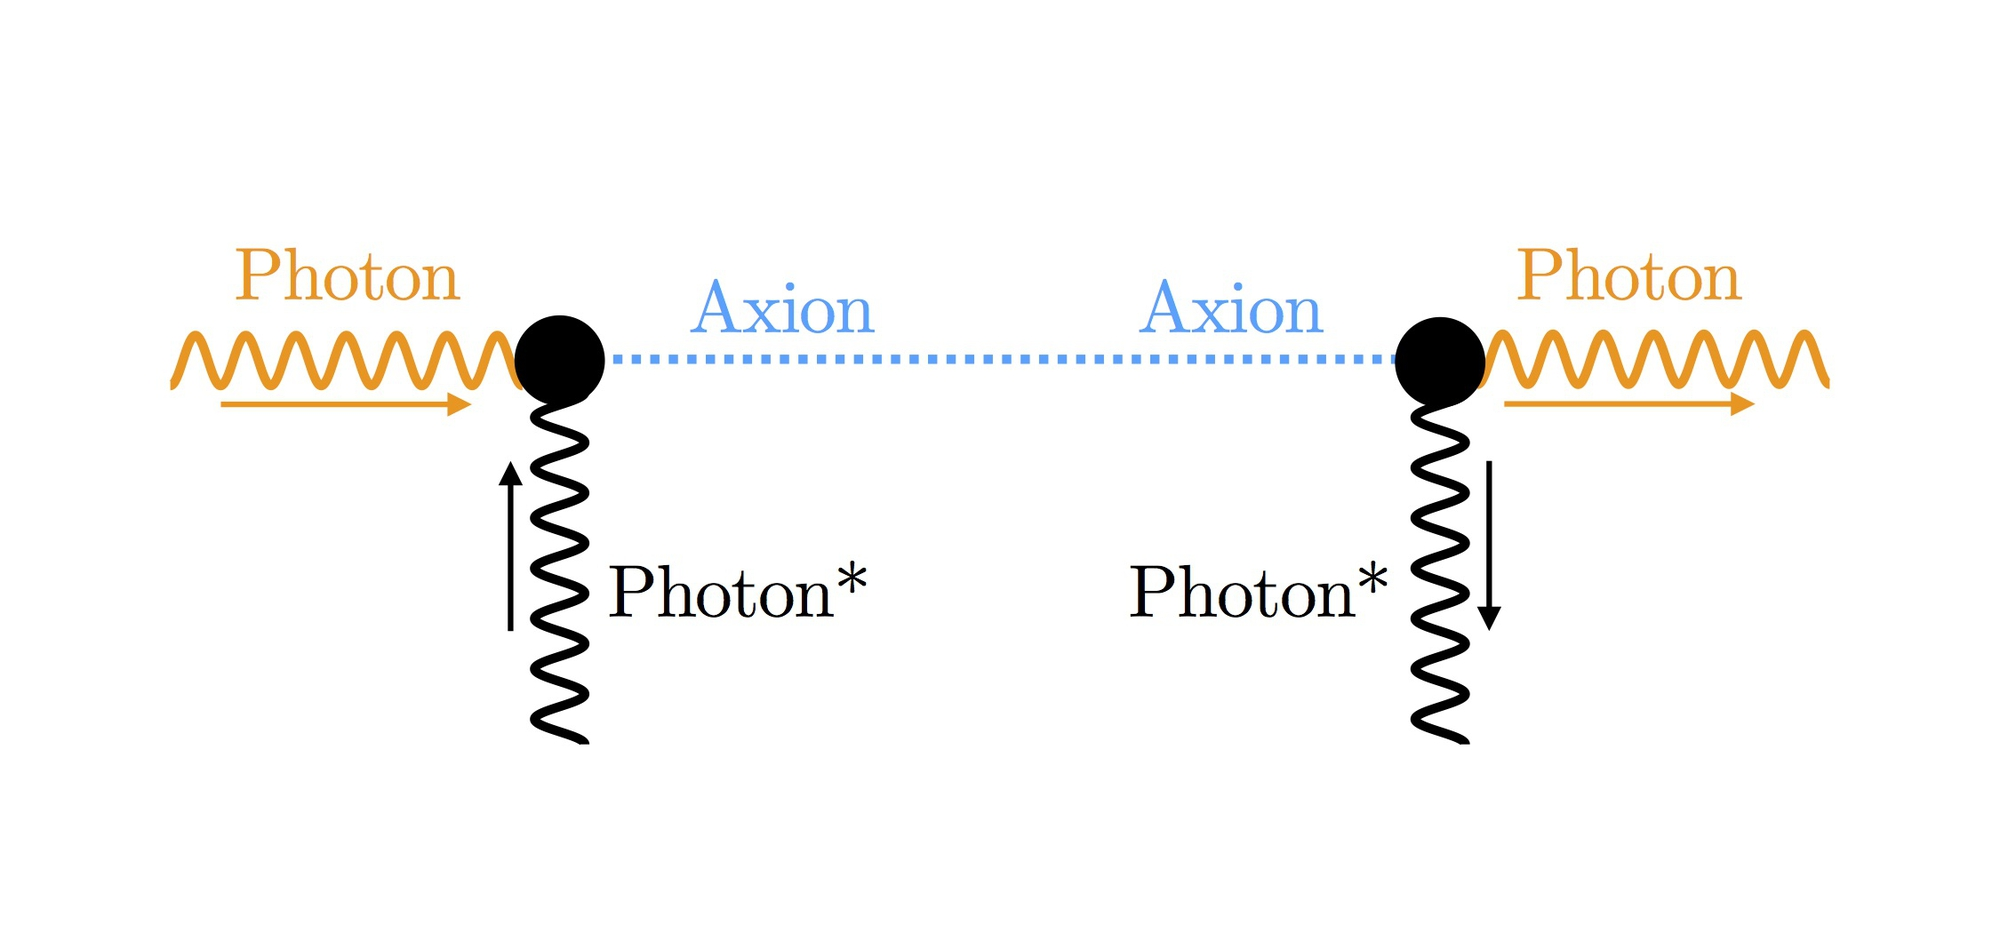
\includegraphics[width=5cm]{img1/axion_photon.jpg}
\end{textblock*}

\begin{textblock*}{4cm}(8.6cm,4.5cm) % {block width} (coords)
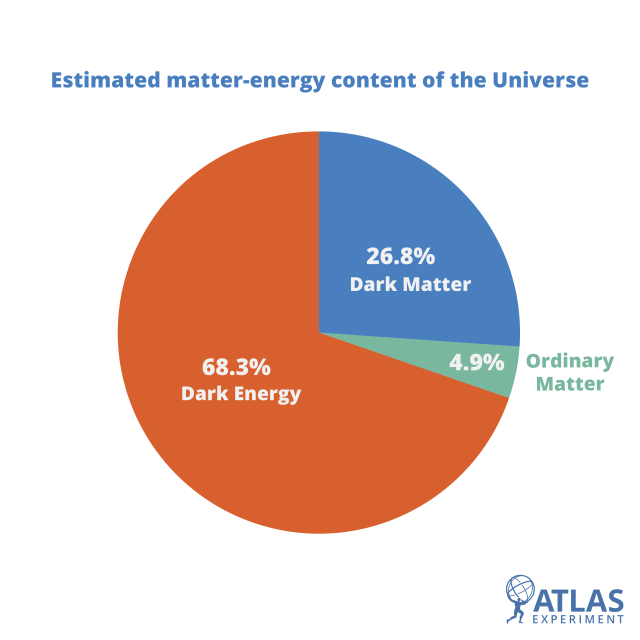
\includegraphics[width=4cm]{img1/pie_chart_DM.png}
\end{textblock*}

\begin{textblock*}{9cm}(0.01cm,2.7cm) % {block width} (coords)
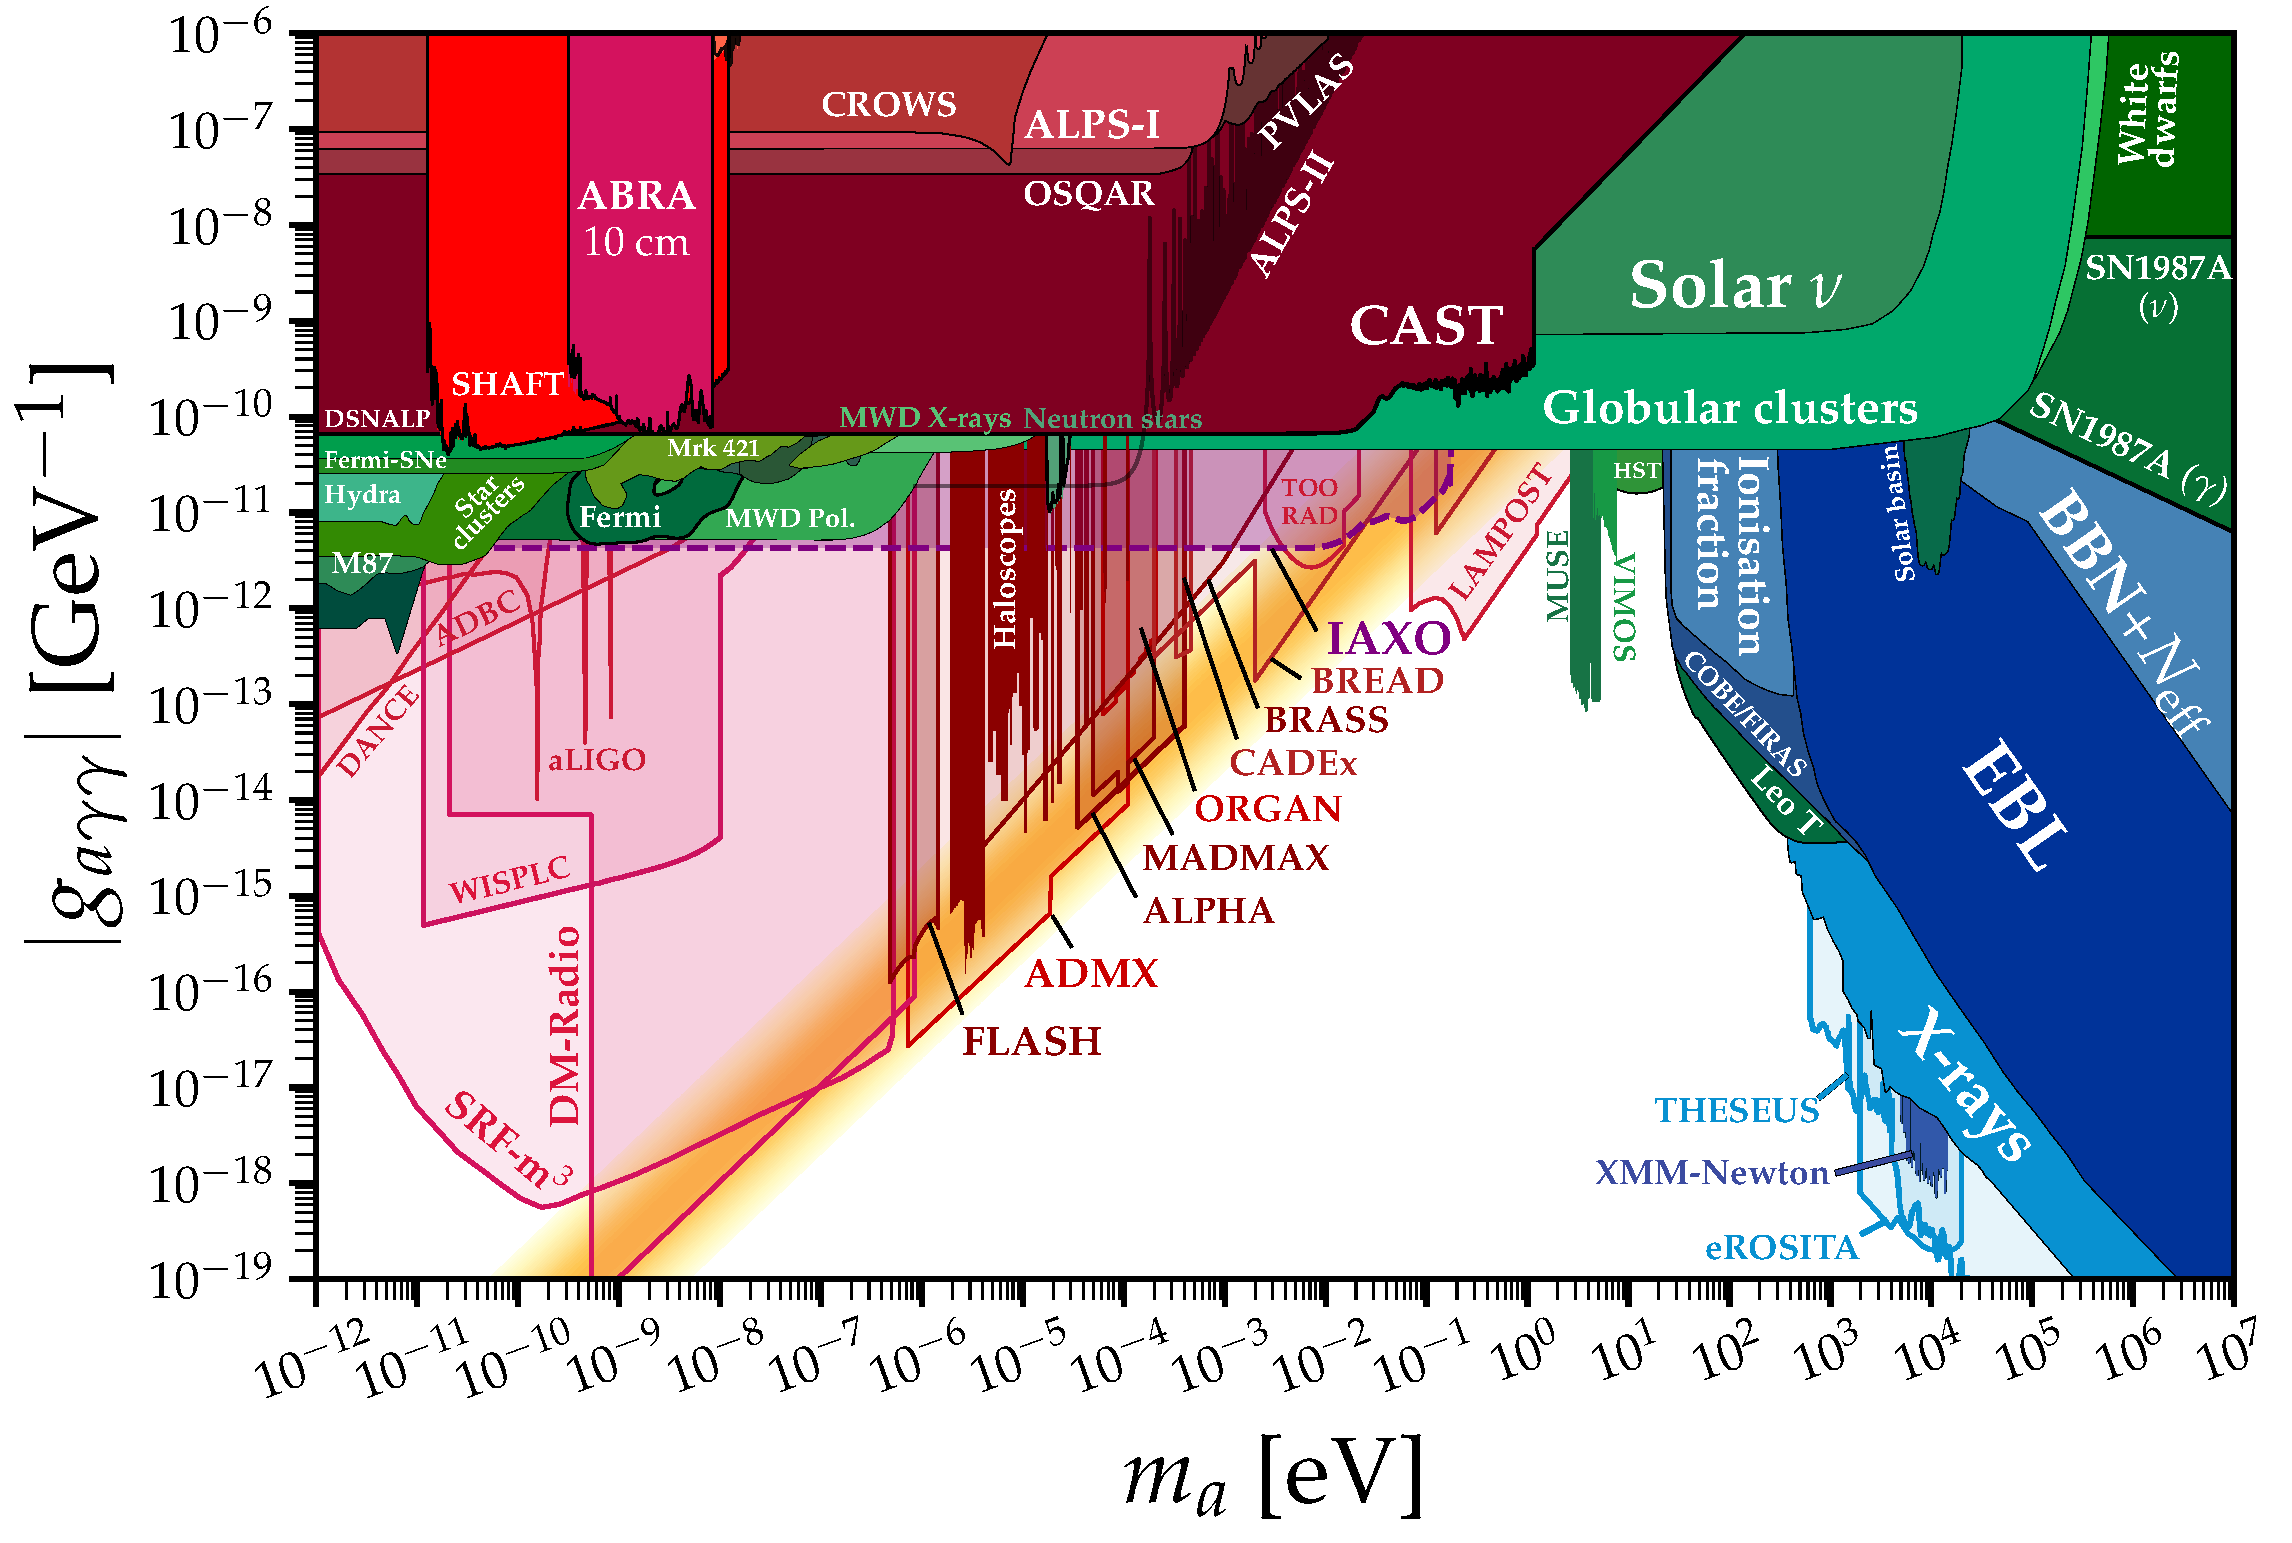
\includegraphics[width=8.4cm]{img1/AxionPhoton_with_Projections.pdf}
\end{textblock*}



\end{frame}

\begin{frame}
\frametitle{Tecniche di rivelazione (Elioscopi, Aloscopi, LSTW)}



\begin{textblock*}{12cm}(0.5cm,1.5cm) % {block width} (coords)
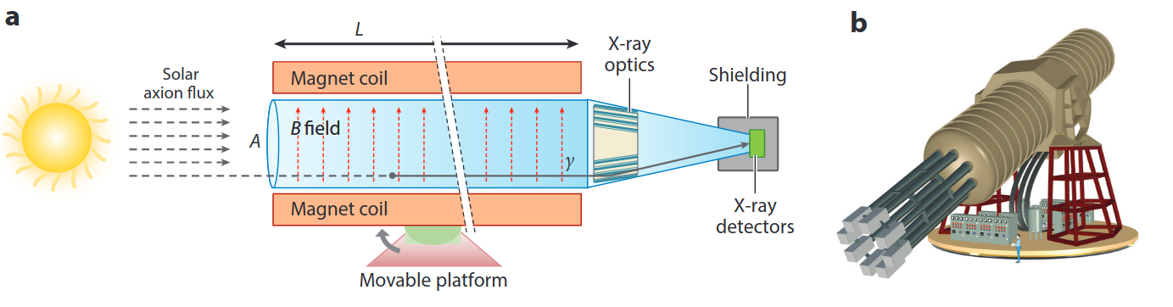
\includegraphics[width=12cm]{img2/helioscope.png}
\end{textblock*}


\begin{textblock*}{10cm}(0.5cm,5.0cm) 
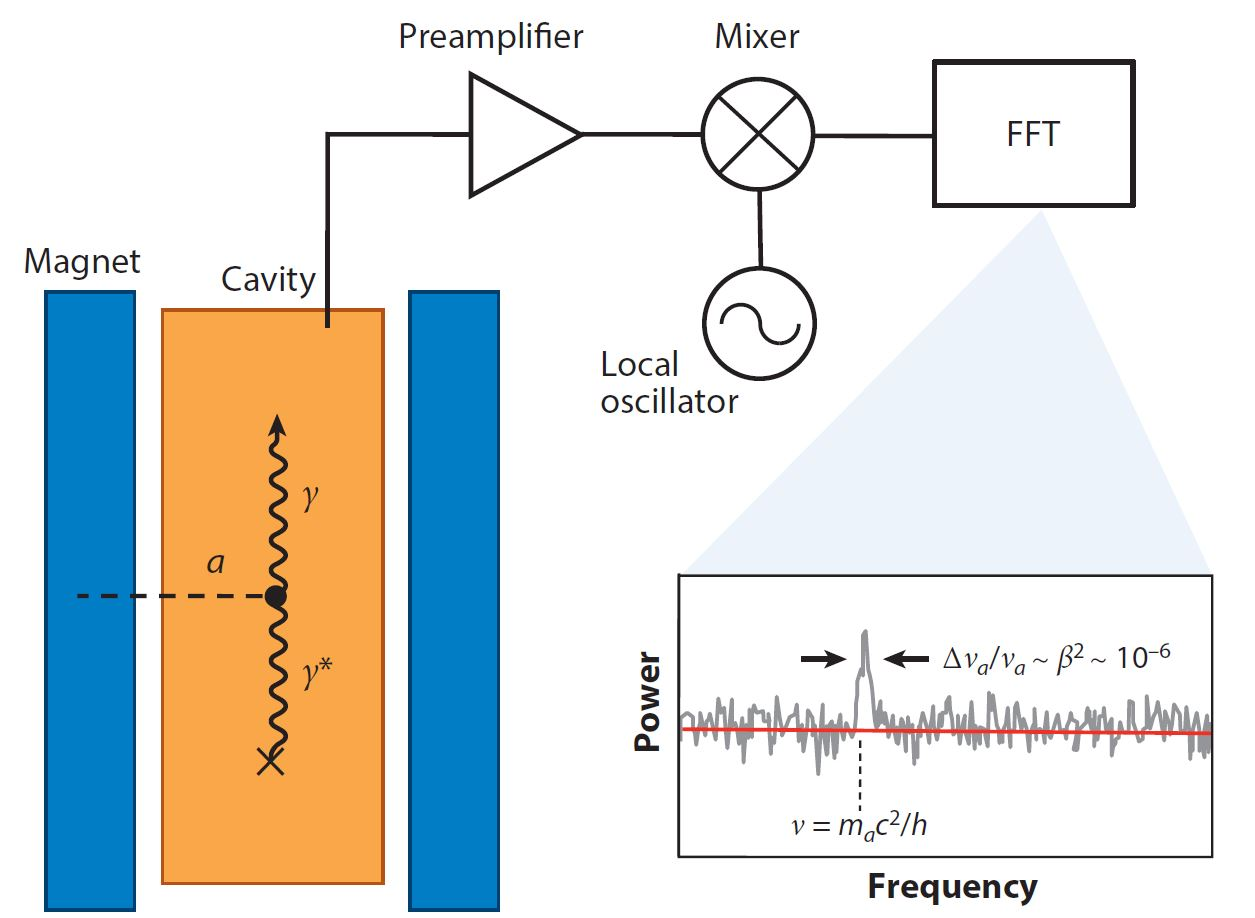
\includegraphics[width=5.0cm]{img2/aloscopio_new.JPG}
\end{textblock*}

\begin{textblock*}{10cm}(5.85cm,5.8 cm) 
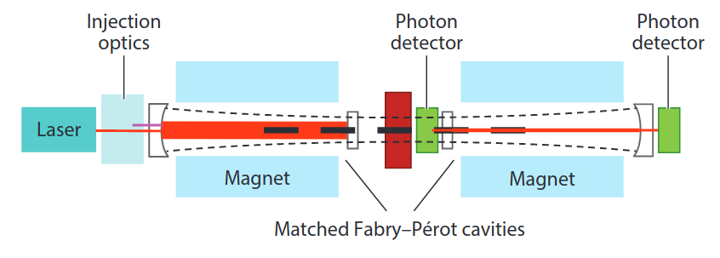
\includegraphics[width=6.8cm]{img2/lstw.png}
\end{textblock*}



\end{frame}


\begin{frame}
\frametitle{Qubit superconduttori e giunzioni Josephson}


\begin{textblock*}{4cm}(1cm,2.8cm) % {block width} (coords)
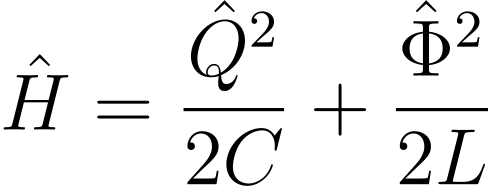
\includegraphics[width=2.5cm]{img3/HLC_new.png}
\end{textblock*}

\begin{textblock*}{4cm}(0.4cm,4cm) % {block width} (coords)
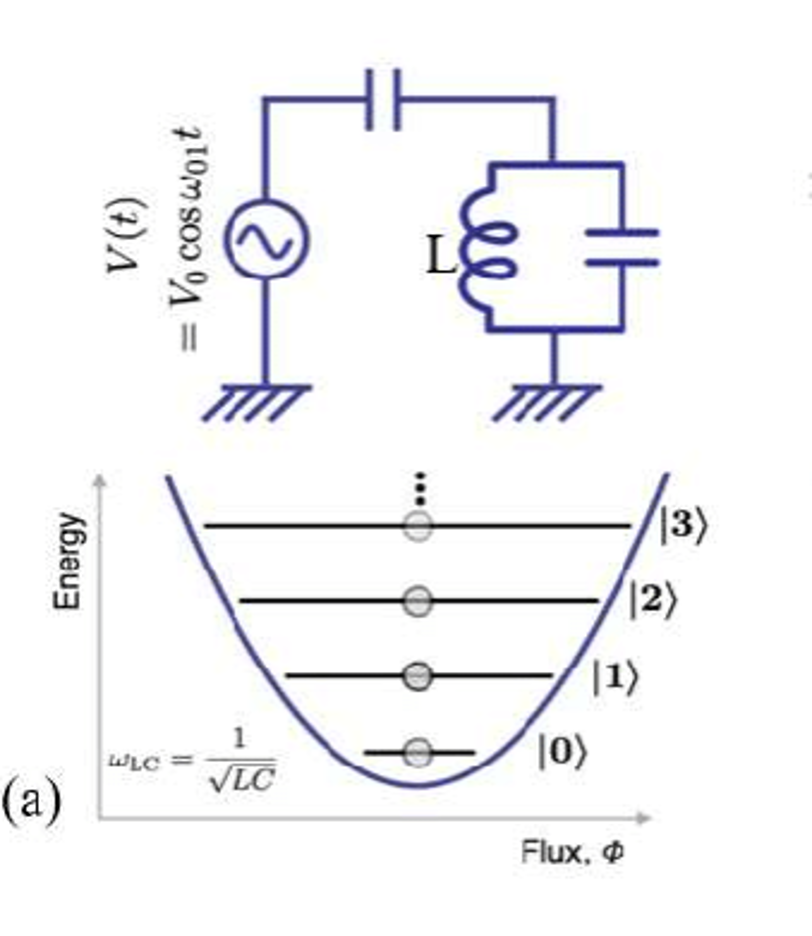
\includegraphics[width=4cm]{img3/LC_microwave.png}
\end{textblock*}

\begin{textblock*}{3.5cm}(4.4cm,2cm) % {block width} (coords)
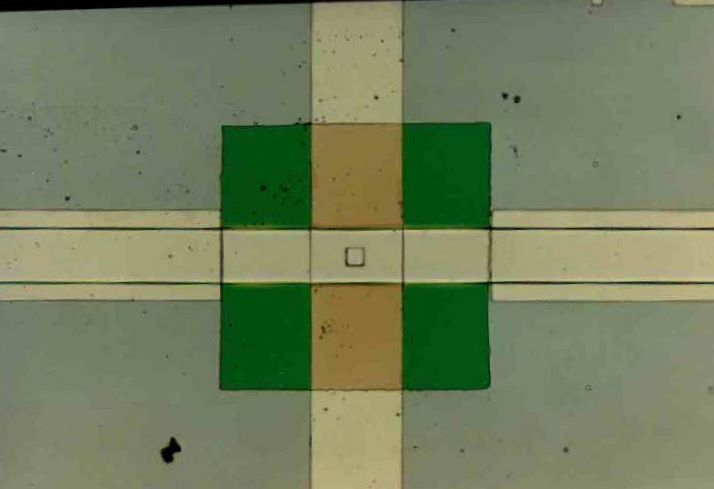
\includegraphics[width=3.5cm]{img3/Josephson_junction_real.jpg}
\end{textblock*}

\begin{textblock*}{3.5cm}(4.4cm,5.1cm) % {block width} (coords)
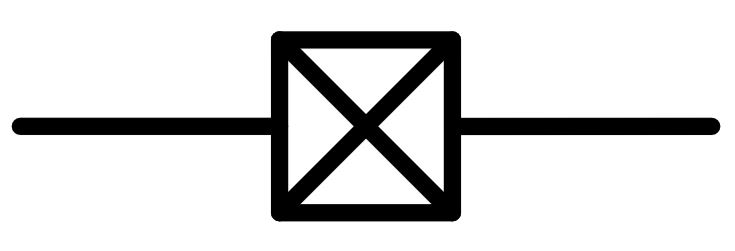
\includegraphics[width=3.4cm]{img3/JJ_simbolo.JPG}
\end{textblock*}


\begin{textblock*}{3.5cm}(4.4cm,7cm) % {block width} (coords)
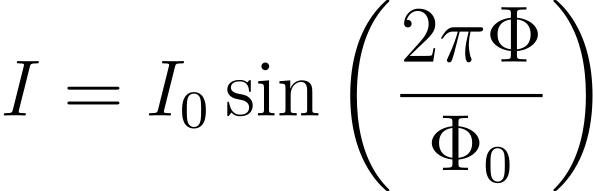
\includegraphics[width=3.4cm]{img3/IJJ_new.png}
\end{textblock*}

\begin{textblock*}{4cm}(8.5cm,4.1cm) % {block width} (coords)
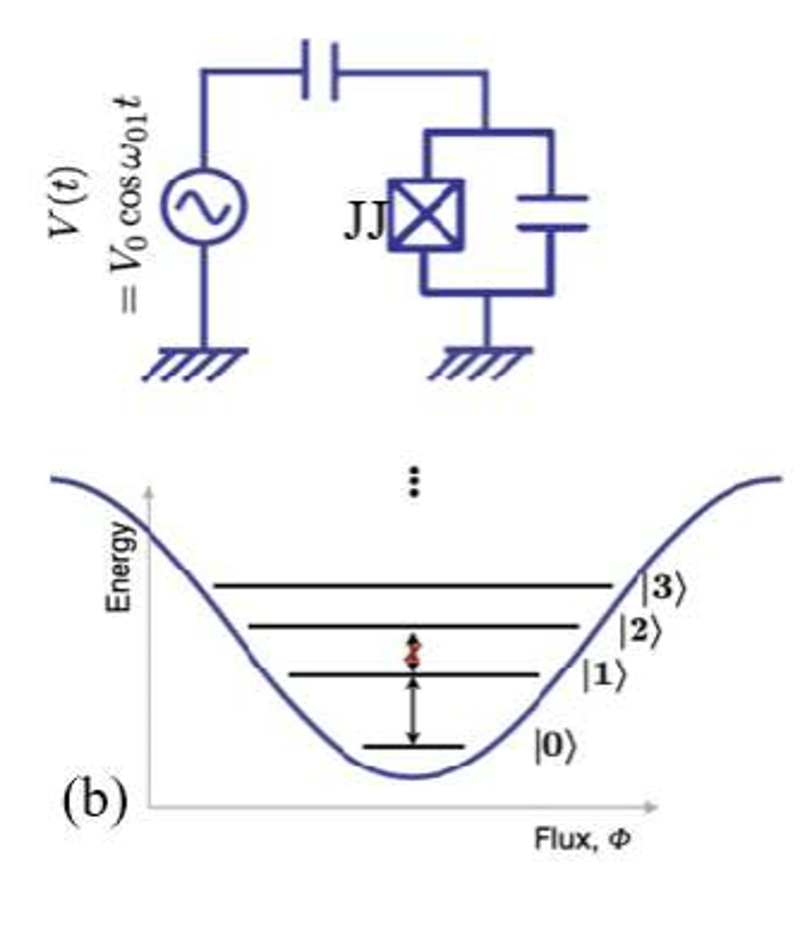
\includegraphics[width=4cm]{img3/JJ_energy.png}
\end{textblock*}


\begin{textblock*}{4cm}(8.3cm,2.8cm) % {block width} (coords)
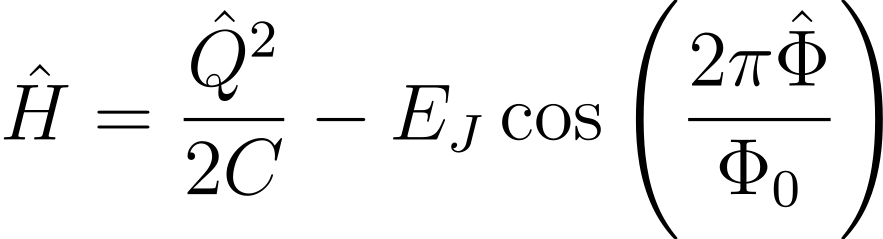
\includegraphics[width=4cm]{img3/HJJ_new.png}
\end{textblock*}


\end{frame}


\begin{frame}[t]
\frametitle{I transmoni}

\centering
\Large $\hat{H}=4E_C(\hat{n}-n_g)^2 - E_J\cos\hat{\varphi}$



\begin{textblock*}{6cm}(0.1cm,3cm) % {block width} (coords)
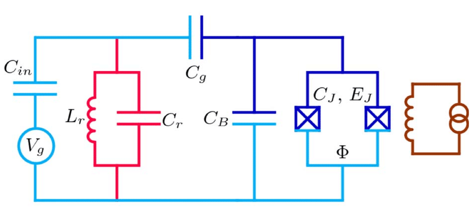
\includegraphics[width=5.5cm]{img4/trasmon.png}
\end{textblock*}


\begin{textblock*}{5.5cm}(0.37cm,6.2cm) % {block width} (coords)
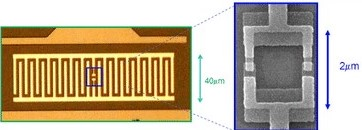
\includegraphics[width=4.7cm]{img4/transmon_SEM.jpg}
\end{textblock*}

\begin{textblock*}{6.5cm}(6.1cm,3.3cm) % {block width} (coords)
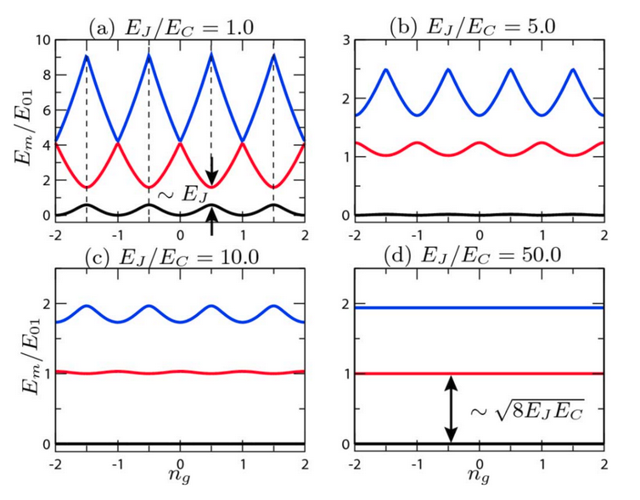
\includegraphics[width=6.5cm]{img4/EJEC.png}
\end{textblock*}


\end{frame}


\begin{frame}[t]
\frametitle{Impiego dei transmoni per la rivelazione dei singoli fotoni nelle microonde \textit{(Qubit-based photon counter)} }


\textbf{\textit{Quantum nondemolition (QND)\\ measurements}:} un nuovo impulso\\ per la ricerca di assioni e non solo...

% \begin{textblock*}{6cm}(0.3cm,2.7cm) % {block width} (coords)
% 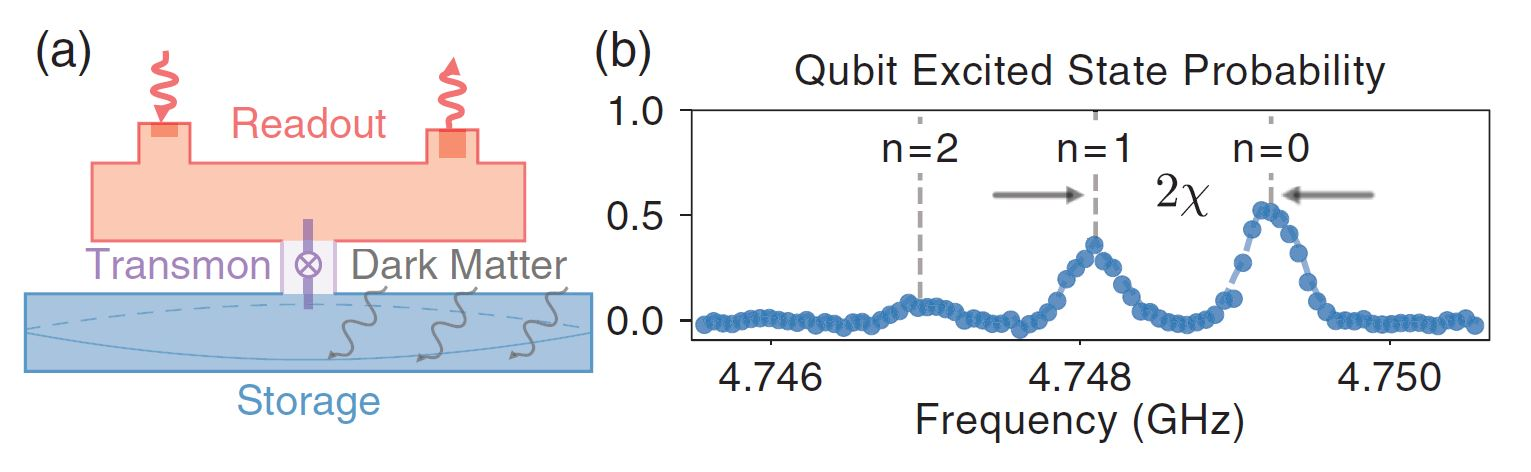
\includegraphics[width=5.5cm]{img5/qubit_freq.JPG}
% \end{textblock*}


\begin{textblock*}{4.5cm}(0.7cm,4.4cm) % {block width} (coords)
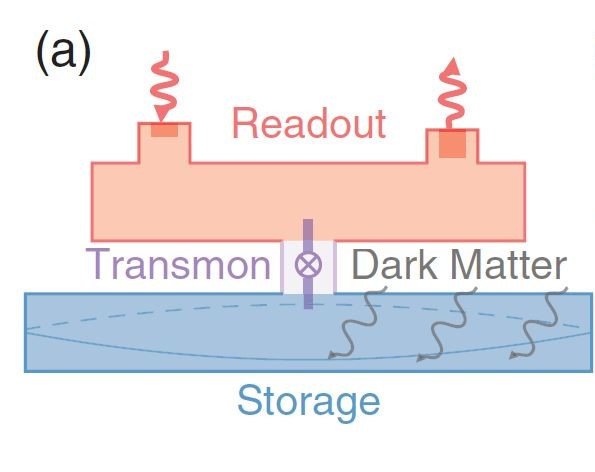
\includegraphics[width=2.8cm]{img5/qubit_freq_a.jpg}
\end{textblock*}


\begin{textblock*}{4.5cm}(0.3 cm,6.9cm) % {block width} (coords)
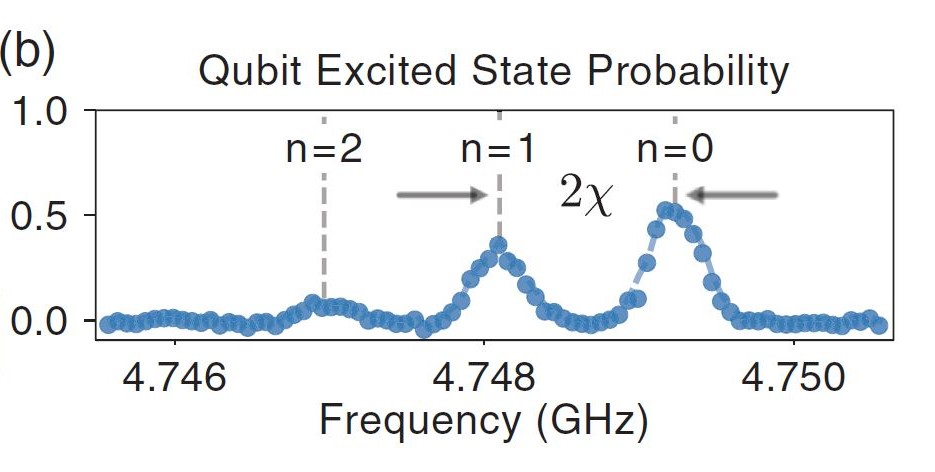
\includegraphics[width=3.5cm]{img5/qubit_freq_b.jpg}
\end{textblock*}

\begin{textblock*}{6.5cm}(6.1cm,2cm) % {block width} (coords)
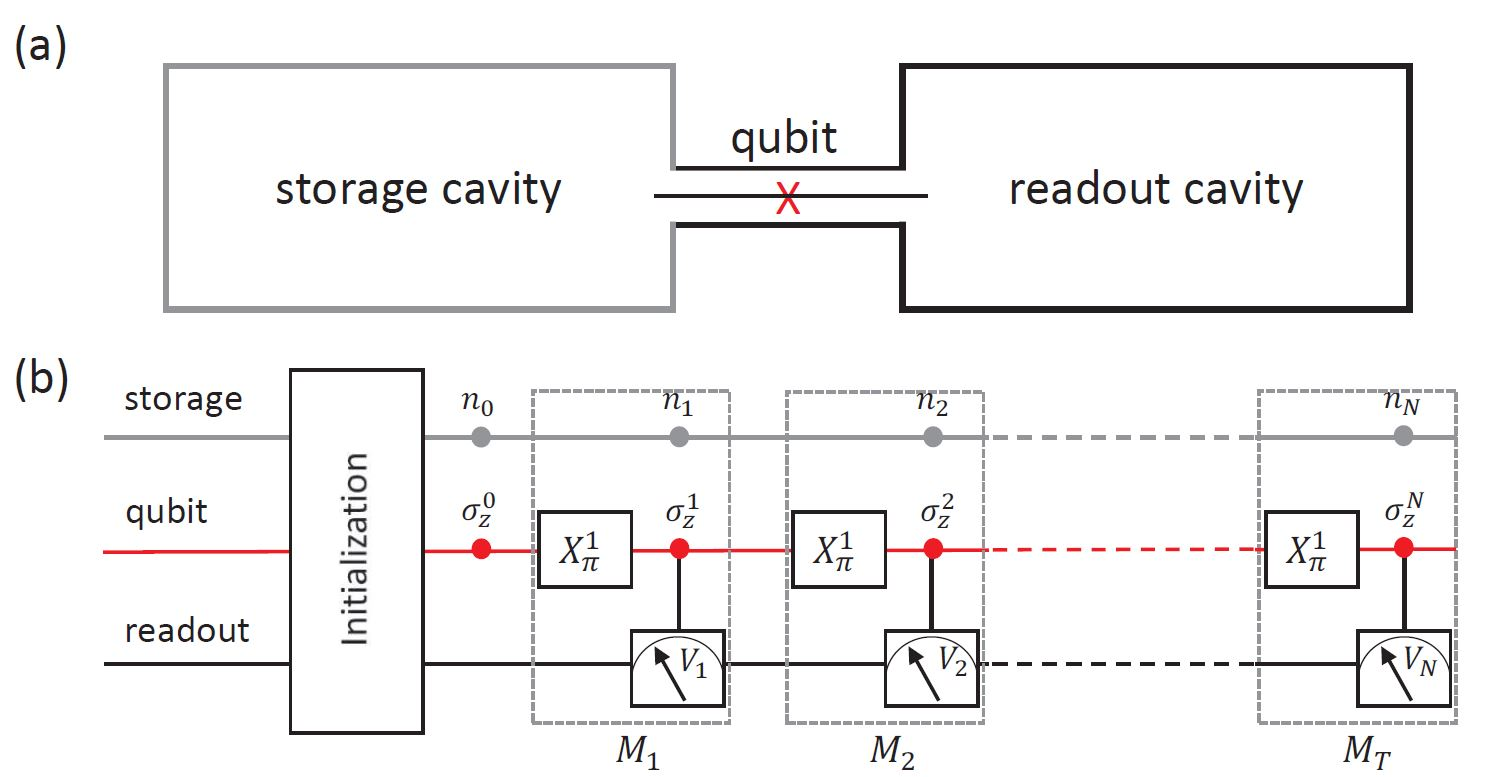
\includegraphics[width=6.3cm]{img5/cavity.JPG}
\end{textblock*}


\begin{textblock*}{10cm}(4.0cm,5.5cm) 
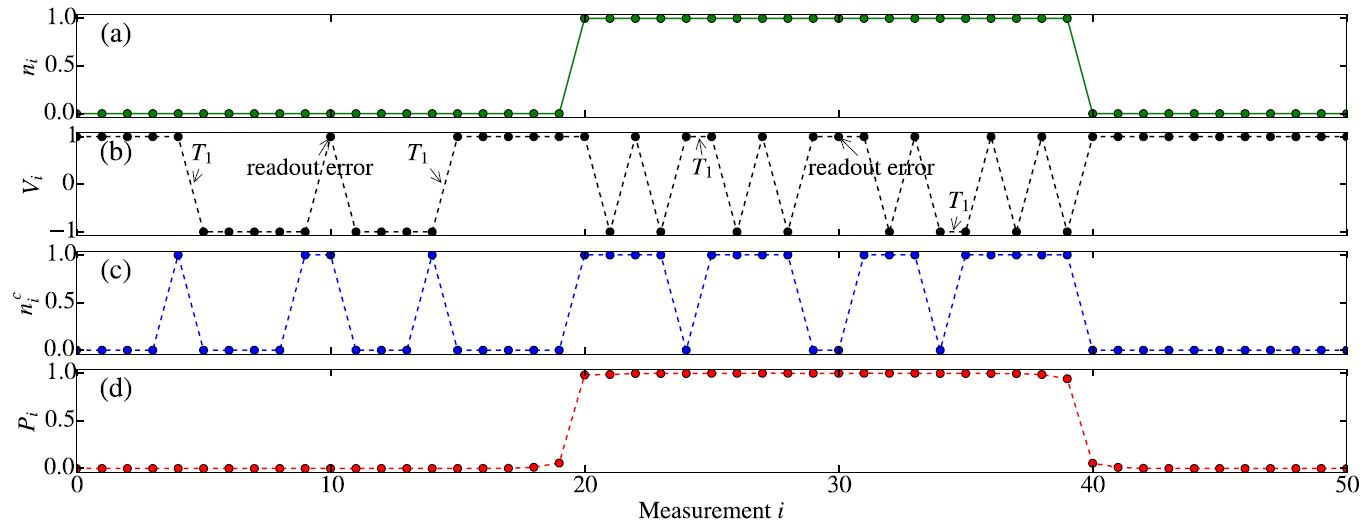
\includegraphics[width=8.4cm]{img5/measures.JPG}
\end{textblock*}

\end{frame}


\begin{frame}
\textcolor{myNewColorA}{\Huge{\centerline{Grazie!}}}
\end{frame}



\begin{frame}[allowframebreaks]
        \frametitle{Bibliografia}
        \bibliographystyle{plain}
        \bibliography{bibliografia.bib}
        \nocite{*}
        \textbf{Fonti Immagini:}\\
        - \url{https://github.com/cajohare/AxionLimits}  by Ciaran O’Hare\\
        
        - \url{https://alps.desy.de/sites/sites_desygroups/sites_extern/site_alps/content/e107103/e101218/e105565/ALPSMAIN101_big.jpg}\\
        
        - \url{https://atlas.cern/updates/feature/dark-matter}\\
        
        
        -\url{https://it.wikipedia.org/wiki/Giunzione_Josephson}\\
        
        - Pashupati Dhakal. Superconducting radio frequency resonators for quantum computing: A short review, 12 2021.\\
        
        - Humble, Travis \& Thapliyal, Himanshu \& Munoz-Coreas, Edgard \& Mohiyaddin, Fahd \& Bennink, Ryan. (2018). Quantum Computing Circuits and Devices. \\

\end{frame}

\end{document}



